\documentclass[12pt]{article}
\input{iati_structure.tex}
\renewcommand{\bottomtitlespace}{3cm}

\usepackage{etoolbox}
\makeatletter
\preto{\@verbatim}{\topsep=0pt \partopsep=0pt }
\makeatother

\begin{document}

\renewcommand{\headerLang}{English}
\renewcommand{\problemName}{A12. Bits and Tree}

\renewcommand{\headerLeft}{IATI Day 1, Senior group}
\renewcommand{\headerRightFirst}{XVI INTERNATIONAL ADVANCED TOURNAMENT IN INFORMATICS}
\renewcommand{\headerRightSecond}{SHUMEN 2025}

\renewcommand{\tl}{$15.00$ s}
\renewcommand{\ml}{$2048$ MB}
\problem{Task \problemName}
\addauthor{Author: Viktor Kozhuharov}{2025}{04}{12}

You are given a binary string \( S \) of length \( 2N \). Your task is to encode the \textbf{longest prefix} you can of \( S \) using an unlabeled undirected tree with \( N \) nodes.

To do this, you need to write two functions: an encoder and a decoder. Your encoder will get the binary string and construct a tree with nodes labeled from \( 0 \) to \( N - 1 \). However, the communication medium is unreliable and will \textbf{corrupt the tree} by adding one extra node and connecting it to one of the original \( N \) nodes. The decoder will receive only this corrupted version of the tree, which now has \( N + 1 \) nodes and \( N \) edges. Additionally, the labels and edges (and the nodes in each edge) will be randomly permuted before being passed to the decoder. This simulates passing an \textbf{unlabeled} tree to the decoder. The decoder must rely only on the structure of the tree and cannot assume anything about the labels.

Your decoder must return a string that shares as long a common prefix as you can with the original string \( S \) \textbf{no matter where the corruption occurred}. Your score will depend on the minimum length of a common prefix among \textit{all possible corruption scenarios} and among all subtests of all tests.

\subsection{Implementation details}

You need to implement the following functions:

\begin{verbatim}
std::vector<std::pair<int, int>> encode(int n, std::vector<bool> data)
\end{verbatim}

This function receives: an integer $N$ ()the number of nodes you are allowed to use) and a boolean vector \texttt{data}, representing the binary string $S$. It should return a list of $N - 1$ edges forming a tree of $N$ nodes (0-indexed).

\begin{verbatim}
std::vector<bool> decode(int n, std::vector<std::pair<int, int>> tree)
\end{verbatim}

This function receives: an integer $N$ (which is the original value passed to \texttt{encode}) and a vector of $N$ edges forming a tree with $N + 1$ nodes (corrupted version). It should return a sequence of bits that should match the original \texttt{data} to as long as prefix as you can.

For a given test, the grader will run $1$ instance of the encoder and $N$ different ones of the decoder. Each of these instances will have its respective function called $T$ times -- once per subtest of the test.

Your program should not implement a \verb|main| function and it should not interact with the standard input and output. It will be compiled together with a system grader that will handle these parts.

\subsection{Constraints}

\begin{itemize}
    \item $ T = 2 $
    \item $ N = 200 $
    \item $|\texttt{data}| = 2 N $
    \item Node labels range from $0$ to $N - 1$ in the uncorrupted tree.
    \item Node labels range from $0$ to $N$ in the corrupted tree.
\end{itemize}

\subsection{Scoring}

Your final score for the task (as a fraction of the full points) is based on the number of correctly decoded bits produced by your solution.

If your solution produces an invalid tree, your score will be 0.

Otherwise, your score \( S \) is computed using the following piecewise linear function:

\begin{adjustbox}{width=1.0\textwidth}
	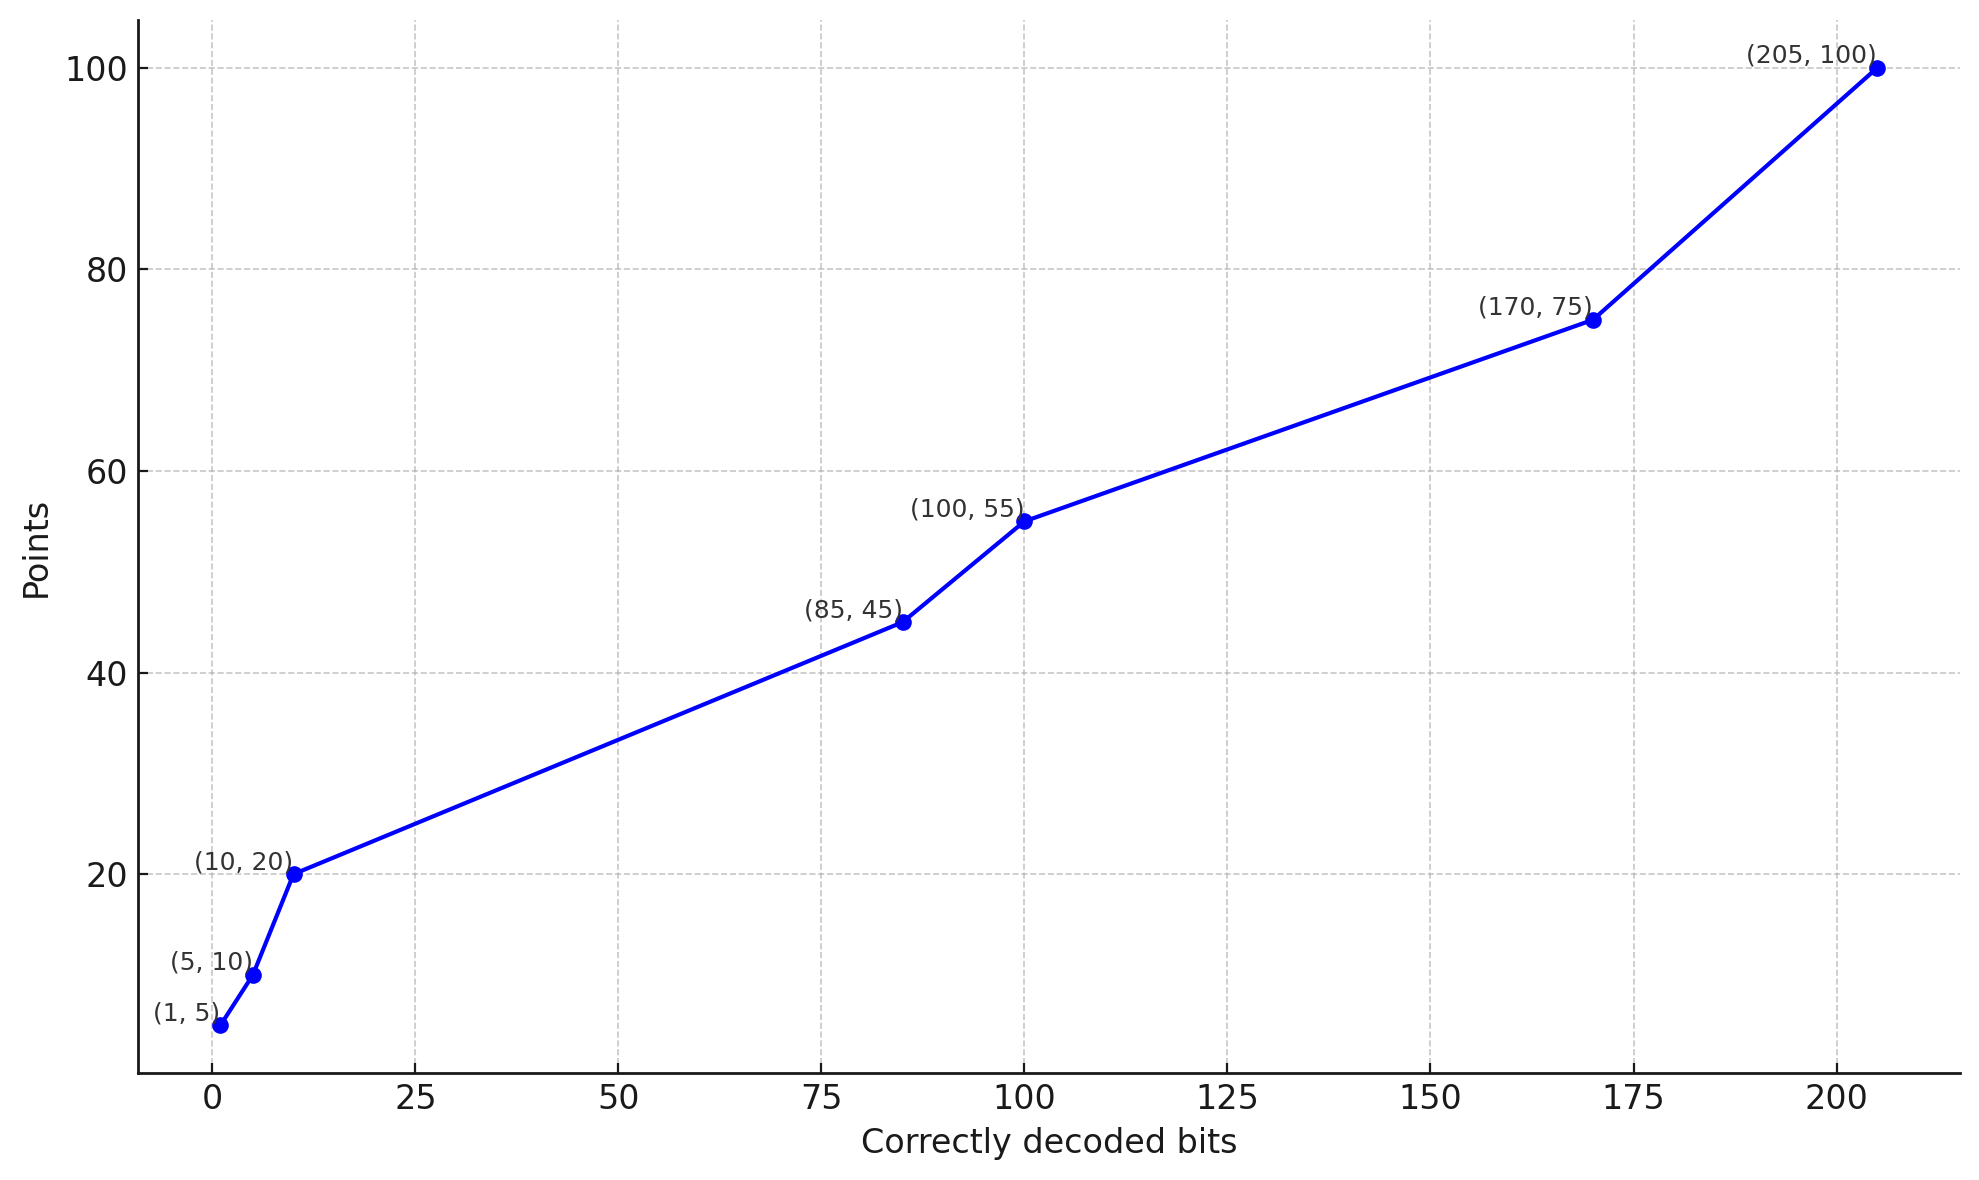
\includegraphics{points_plot}
\end{adjustbox}

The number of correctly decoded bits is the minimum among all tests, subtests, and corruption scenarios.

\newpage

\subsection{Local Testing}

A local grader is provided to help you test your solution. It needs to be compiled together with your program. It does not use separate processes.

It simulates the full encoding/decoding pipeline:

\begin{enumerate}
    \item Reads an integer $T$ -- the number of subtests.
    \item For each test case:
    \begin{enumerate}
        \item Reads an integer $N$ -- the number of nodes available for encoding.
        \item Reads an integer $\ell$ -- the length of the binary data string (usually $2N$).
        \item Reads $\ell$ bits (each $0$ or $1$ without spaces) representing the binary string $S$.
        \item Calls your \verb|encode(n, data)| function.
        \item Tries corrupting the resulting tree by:
        \begin{itemize}
            \item Iterating through each $x$ — the index of the node (from $0$ to $N-1$) to attach a new node to. \vspace{0.4em}
            \item Adds a new node and attaches it to node $x$. \vspace{0.4em}
            \item Randomly permutes the node labels, shuffles the edge lists and swaps at random the 2 ends of each edge. \vspace{0.4em}
        \end{itemize}
        \item Calls your \verb|decode(n, corrupted_edges)| function with each corrupted tree.
        \item Compares each result against the original data and counts how many bits match the original string in the shortest matching prefix.
    \end{enumerate}
\end{enumerate}

\subsubsection*{Example Interaction}
\begin{table}[H]
\begin{tblr}{|l|X[j]|}
\hline
\textbf{Input} & \textbf{Interaction} \\
\hline
\texttt{\makecell[lt]{1 \\
5 10 1101010110
}}
& 
\texttt{\makecell[lt]{encode(5, \{1,1,0,1,0,1,0,1,1,0\}) \\
returns \{\{0,1\},\{1,2\},\{0,3\},\{1,4\}\} \\
decode(5, \{\{1,0\},\{0,2\},\{2,3\},\{3,4\},\{5,3\}\}) \\
returns \{1,1,0\} \\
decode(5, \{\{1,0\},\{0,2\},\{0,3\},\{4,0\},\{5,4\}\}) \\
returns \{1,1,1,0,1,0,1,0\} \\
decode(5, \{\{2,0\},\{2,1\},\{1,3\},\{4,1\},\{5,4\}\}) \\
returns \{1,1,1,0,0,0,0,0\} \\
decode(5, \{\{0,1\},\{0,2\},\{0,3\},\{4,3\},\{3,5\}\}) \\
returns \{1,1,1,0,1\} \\
decode(5, \{\{1,0\},\{1,2\},\{2,3\},\{4,2\},\{5,4\}\}) \\
returns \{1,1,1,0\} \\
}} \\
\hline
\end{tblr}
\end{table}

\begin{verbatim}
\end{verbatim}

\end{document}
